% Theoretical background
%\clearpage % Uncomment if needed to force a page break before the chapter
\vspace{21.5pt}
\chapter{Teoreettinen tausta}

Jotta voidaan tutkia sitä, miten funktionaalinen ohjelmointi vaikuttaa ohjelmointiin \gls{ts} ympäristössä, on kartoitettava mitä ylipäätään funktionaalinen ohjelmointi on.

Teoriaosuudessa pyritään avaamaan funktionaalisen ohjelmoinnin perusteet \glsdisp{language_agnostic}{kieliagnostisesti}, ja toisaalta myös JavaScript- sekä TypeScript-ekosysteemien kannalta.

Teoriaosuuden lopussa pohjustuksen jälkeen voidaan vielä vertailla sitä, miten funktionaalinen ohjelmointi, olio-ohjelmointi, tai proseduraalinen ohjelmointi eroavat käytännössä.

Lopulta näillä tiedoilla voidaan lähteä tutkimaan miten funktionaalisen ohjelmoinnin käytänteet näkyvät hyödyllisesti tai haitallisesti ohjelmistoprojekteissa.

\section{Funktionaalinen ohjelmointi}

Funktionaalinen ohjelmointi on ohjelmointiparadigma, jonka juuret ulottuvat 1930-luvulle ja lambda-kalkyylin kehitykseen. Lähestymistapa korostaa funktioiden käyttöä perusyksikköinä ja pyrkii välttämään muuttuvia tiloja sekä sivuvaikutuksia. Funktionaalisen ohjelmoinnin keskeisiä käsitteitä ovat \glsdisp{pure_function}{puhtaat funktiot}, \glsdisp{higher_order_function}{korkeamman asteen funktiot}, \gls{immutable_data} sekä \gls{declarative_programming}. \citep{Tan2004,computerphile_lambda}

\subsection{Nimeämiskäytänteet}

Ohjelmoidessa funktionaalista ohjelmakoodia nimeämiskäytänteet ovat yhtä vaikeita kuin aina. Tässä insinöörityössä käytetään Haskell-ohjelmoijien keskuudessa näkyviä nimeämiskäytänteitä, jossa käytetään lyhyitä ja \textquote{intuitiivisia} nimiä funktioille ja muuttujille. Esimerkiksi:

\begin{itemize}
    \item x: Yleisesti käytetty muuttuja tai parametri, joka edustaa arvoa, jota funktiot käsittelevät. Jos näkyvyys-alalla on muita funktioita, niitä nimetään usein aakkosjärjestyksessä x:stä eteenpäin (x, y, z).
    \item xs: Muuttuja, joka edustaa useita arvoja (useita x-kirjaimia). Usein sisältää listan arvoista, mutta tietorakenteen tietäminen ei ole merkittävää.
    \item f: Yksittäinen funktio, jota voidaan käyttää käsittelemään arvoja. Jos näkyvyys-alalla on muita funktioita, niitä nimetään usein aakkosjärjestyksessä f:stä eteenpäin (f, g, h, i...).
    \item fs: Muuttuja, joka edustaa useita funktioita (useita f-kirjaimia). Usein sisältää listan funktioista, mutta tietorakenteen tietäminen ei ole merkittävää.
\end{itemize}

Esimerkkejä käytänteiden käytöstä:

\begin{code}
    \begin{minted}{javascript}
const map    = f => xs => xs.map(f)
const either = f => g => x => f(x) || g(x)
const max    = x => y => x > y ? x : y
const pipe   = fs => x => fs.reduce((acc, f) => f(acc), x)
\end{minted}
    \caption{Esimerkkejä insinöörityössä käytettävistä nimeämiskäytänteistä.}
    \label{code:javascript_naming_convention_example}
\end{code}

\subsection{Kombinaattorit}


Funktionaalinen ohjelmointi mahdollistaa koodin uudelleenkäytettävyyden. Lambda-kalkyylin perustein joka ikisien ongelman voi purkaa pieniksi funktioiksi. \citep{BlellochHarper2015} Lambda-kalkyylin voi ajatella olevan esoteerinen ohjelmointikieli. Sen voi kuitenkin myös ottaa osaksi ohjelmoijan työkalupakkia missä tahansa ohjelmointikielessä, joka kohtelee funktioita ensiluokkaisina, eli siten, että niitä voi käyttää muuttujina (Koodiesimerkki \ref{code:javascript_combinators}).

Kombinaattorit ovat omalla tavallaan sitä, mitä suunnittelumallit ovat olio-ohjelmoinnissa: tapa ratkaista ongelmia yleisesti ja siten, että siitä voidaan keskustella.

\begin{code}
    \begin{minted}{javascript}

const identity      = x => x
const constant      = x => y => x
const apply         = f => x => f (x)
const thrush        = x => f => f (x)
const duplication   = f => x => f (x) (x)
const flip          = f => y => x => f (x) (y)
const compose       = f => g => x => f (g (x)) 
const substitution  = f => g => x => f (x) (g (x))

\end{minted}
    \caption{Yleiset kombinaattorit esitettynä JavaScriptissä \cite{javascript_combinators}. Kombinaattoreilla voi esittää lambda-kalkyyliä, ja ohjelmoida Turing-vahvoja ohjelmia.}
    \label{code:javascript_combinators}
\end{code}

Kombinaattorit näyttävät uhkaaviilta ja raa'assa muodossaan niiden hyötyarvoa voi olla hankala havaita. Niiden käyttämistä voi kuitenkin perustella niiden perustavanlaatuisten ja kieliagnostisien ominaisuuksien takia. Ohjelmoidessa funktionaalisesti ei kombinaattoreita kuitenkaan tarvitse paljoa ajatella. Niitä tulee kirjoittamaan varmasti vähintään vahingossa, sillä niitä vaaditaan funktioita pyörittäessä. Kuitenkin on hyvä tiedostaa käytössä olevat rakennuspalikat, ja millä nimellä etsiä niistä tietoa tarvittaessa.




\subsection{Yhdistefunktiot ja niiden vahva merkitys}

Usein funktionaalista ohjelmointia mainostaessa puhutaan funktioiden puhtauden ja datan muuttumattomuuden olevan paradigman oleellisinta. Kuitenkin samaan aikaan juuri datan muuttumattomuus ja tilattomuus koetaan paradigman suureksi kompastuskiveksi \cite{cantarella_fp_haitat,is_reduce_bad,vakil2016}.

On tärkeää huomata, että kaiken ei tarvitse olla täysin puhdasta ja muuttumatonta, kunhan ne osat, joissa funktionaalista ohjelmointia hyödynnetään, pysyvät ennustettavina ja hallittavina.

\Glspl{composed_function} ovat loistava tapa kirjoittaa selkeää ja modulaarista koodia. Parasta on, että kaiken ei tarvitse olla pelkkiä funktioita: voi hyvin kirjoittaa myös olio-ohjelmointityylillä ja silti hyödyntää yhdistefunktioita logiikan selkeyttämiseksi ja yksinkertaistamiseksi.

Loppujen lopuksi funktionaalisen ohjelmoinnin perusta on funktioissa ja niiden yhdistämisessä. Datan muuttumattomuus ja sivuvaikutuksettomuus on vain esivaatimus funktioiden ennustettavuudelle.

\Gls{composed_function} tarkoittaa yksinkertaisesti kahden tai useamman funktion yhdistämistä siten, että yhden funktion tulos syötetään seuraavalle. Esimerkiksi funktion f(g(x)) voi nähdä kahden funktion f ja g yhdisteenä, jossa g suoritetaan ensin ja sen tulos annetaan funktiolle f (Koodiesimerkki \ref{code:javascript_manual_composition}).

\begin{code}
    \begin{minted}{javascript}
const f = x => 2 * x

const g = x => x + 3

const h = x => f(g(x))
\end{minted}
    \caption{JavaScript-esimerkki yhdistetystä funktiosta h ilman pipe tai compose funktiota}
    \label{code:javascript_manual_composition}
\end{code}

Funktionaalisissa ohjelmointikielissä yhdistettyjä funktioita pystyy usein kirjoittamaan käyttäen kieleen sisäänrakennettuja operaattoreja, joilla koostaminen on helpompaa ja suoraan osana ohjelmointikieltä \cite{fsharpcomposition,haskellcomposition}.
JavaScriptissä ei ole vastaavanlaista sisäänrakennettua operaattoria.
(Vaikkakin sellainen on kehitteillä \cite{tc39_pipeline_operator})
Operaattorin voi kuitenkin kirjoittaa helposti itse funktiona (Koodiesimerkki \ref{code:javascript_pipe_composition}).

\begin{code}
    \begin{minted}{javascript}
const pipe    = f => g => x => g(f(x))
const compose = f => g => x => f(g(x))

const h = pipe(f)(g)
// tai vaihtoehtoisesti
const h = compose(g)(f)
\end{minted}
    \caption{JavaScript-esimerkki funktiokompositiosta pipe ja compose funktioilla}
    \label{code:javascript_pipe_composition}
\end{code}

Voi olla mielenkiinoista huomata, että Koodiesimerkin \mintinline{javascript}{compose} löytyy myös aiemmin mainituista tunnetuista kombinaattoreista (Koodiesimerkki \ref{code:javascript_combinators}).

Koodiesimerkissä on näytettynä kaksi eri tapaa yhdistää funktioita: \mintinline{javascript}{pipe} ja \mintinline{javascript}{compose}. Käytännössä ainoa ero on se, kummasta suunnasta funktiot suoritetaan. \mintinline{javascript}{compose} on lähempänä yhdistettyjen funktioiden matemaattisia perusteita, kun taas \mintinline{javascript}{pipe} on usein helpompi lukea, sillä se suoritetaan yleisessä lukemissuunnassa, eli vasemmalta oikealle, tai ylhäältä alas. Tulevissa koodiesimerkeissä tullaan suosimaan funktioiden yhdistämistä käyttäen \mintinline{javascript}{pipe}-funktiota \mintinline{javascript}{compose}-funktion sijaan. \citep{whyprefercompose}

Esimerkin \mintinline{javascript}{pipe} ja \mintinline{javascript}{compose} toimivat vain kahdelle funktiolle kerrallaan. Tämä tapa seuraa lambda-kalkyyliä \cite{computerphile_lambda}. Eri ohjelmointikielestä riippuen on kuitenkin mieluisaa kirjoittaa funktiot niin, että ne tukevat suoraan mielivaltaista määrää funktioita.

JavaScriptissä näin voi tehdä esimerkiksi hyödyntämällä Array-tietorakennetta (Koodiesimerkki \ref{code:javascript_better_pipe}).

\begin{code}
    \begin{minted}{javascript}
const pipe    = fs => x => fs.reduce((acc, f) => f(acc), x)
const compose = fs => x => fs.reduceRight((acc, f) => f(acc), x)

const f = x => x + 1
const g = x => x * 2
const h = x => x - 3

const i = pipe([f, g, h])
i(5) // (((5 + 1) * 2) - 3) = 9
// tai vaihtoehtoisesti 
const i = compose([h, g, f])
i(5) // (((5 + 1) * 2) - 3) = 9
\end{minted}
    \caption{JavaScript-esimerkki yhdistetystä funktiosta käyttäen reduce ja reduceRight funktioita}
    \label{code:javascript_better_pipe}
\end{code}

Mikä tästä sitten tekee loistavaa? Se, että ohjelmointi on kerrankin oikeasti kuin LEGO palikoilla leikkimistä (Koodiesimerkki \ref{code:javascript_composition_example}).

\begin{code}
    \begin{minted}{javascript}
const pipe     = fs => x => fs.reduce((acc, func) => func(acc), x)
const multiply = x => y => x * y
const add      = x => y => x + y
const filter   = f => xs => xs.filter(f)
const map      = f => xs => xs.map(f)
const isEven   = x => x % 2 === 0

const rejectOdds   = filter(isEven)
const multiplyBy10 = multiply(10)

const pipeline = pipe([rejectOdds, map(multiplyBy10)])

pipeline([1, 2, 3, 4]) // [20, 40]

\end{minted}
    \caption{Käytännöllinen JavaScript-esimerkki funktioiden käyttämisestä koostamiseen}
    \label{code:javascript_composition_example}
\end{code}

Esimerkissä näytetyt funktiot ovat hyvin yksinkertaisia. Kuitenkin ne ovat täysin uudelleenkäytettäviä. Jos totuttautuu käyttämään joitain funktioita kaikissa projekteissa, voi huomata koodin kirjoittamisen tehokkuuden ja johdonmukaisuuden kasvavan.

\section{Joukko-oppi}

Ohjelmointi on aina ollut matemaattista.

\subsection{Joukko-tietorakenne}

Olio-ohjelmoinnissa, tai ylipäätään ohjelmoinnissa, joukko-oppi näkyy ohjelmoijalle yleensä joukko-tietorakenteen muodossa. Jopa JavaScriptissä on sisäänrakennettu joukko-tietorakenne \cite{mdn_set}.

Joukko-tietorakenne kuvaa joukko-opin joukkoa. Käytännössä joukko-tietorakenteessa säilytetään kokoelma uniikkeja alkioita. Joukko-tietorakenne on ohjelmoinnissa mieluinen työkalu sen tehokkuuden ansiosta \cite{ecma_spec}.

Kokemusten mukaan ohjelmoija ei usein mieti joukko-tietorakennetta matemaattisista lähtökohdista. Tästä kuitenkin voisi olla hyötyä.



\subsection{Siirtyminen joukoista toisiin}
Jos joukko-oppia rupeaa miettimään ohjelmoinnissa siirtyminä joukoista toisiin, saa kieliagnostista osaamista kirjoittaa koodia. Kun miettii, mitä ylipäätään voi laskea, pääsee ohjelmoinnissa omalle abstraktille tasolle. \citep{Tan2004,BlellochHarper2015}

Tarkastellaan seuraavia tilanteita.

\begin{code}
    \begin{minted}{typescript}
const add10 = x => x + 10  
\end{minted}
    \caption{Funktio, joka ottaa numeron ja lisää siihen 10}
    \label{code:ts_set_theory_1}
\end{code}

Funktio ottaa numeron ja lisää siihen 10 lisää. Toiminnon käyttökohteita voisi olla esimerkiksi jonkin pistemäärän päivittäminen tai ajan lisääminen. On hyvä näin. Ei mietitä joukko-oppia, vaikka ehkä kannattaisi.

Siirrytään askelta monimutkaisempaan toimintoon: jakamiseen.


\begin{code}
    \begin{minted}{typescript}
const divide = x => y => x / y
\end{minted}
    \caption{Funktio, joka jakaa numeron toisella}
    \label{code:ts_set_theory_3}
\end{code}

Funktio ottaa kaksi numeroa, ja jakaa ensimmäisen toisella. Mutta entä jos toinen annettu numero onkin nolla? Ohjelmointi ei vastaa tähän kysymykseen suoraan, ja se jättää ongelman ohjelmoijan ratkaistavaksi.

Ohjelmoijan toisin sanoen tulisi tietää, että nollalla ei voi jakaa, ja että jos niin kuitenkin tehdään, JavaScript palauttaa arvon \mintinline{javascript}|Infinity| (tai erityisemmässä tapauksessa \mintinline{javascript}|NaN|) (Koodiesimerkki \ref{code:ts_division}).

\begin{code}
    \begin{minted}{typescript}
console.log(1/0)  // Infinity
console.log(1/-0) // -Infinity
console.log(0/0)  // NaN
\end{minted}
    \caption{Jakamisoperaattorin toiminta JavaScriptissä}
    \label{code:ts_division}
\end{code}

Tehdään funktiosta turvallisempi lisäämällä siihen tarkistus.


\begin{code}
    \begin{minted}{typescript}
const divide = x => y => y !== 0 ? x / y : null
\end{minted}
    \caption{Turvallisempi funktio, joka jakaa numeron toisella}
    \label{code:ts_set_theory_4}
\end{code}

Tässä versiossa jakaminen suoritetaan vain, jos jakaja ei ole nolla. Jos jakaja on nolla, palauttaa funktio arvon \mintinline{JavaScript}|null|. Versio ratkaisee ongelman siitä, mitä tapahtuu, jos nollalla satutaan jakamaan. Toisaalta funktio ei kuitenkaan aina palauta numeroa.

Mutta kuinka sitten joukko-oppi? Kuinka se liittyy tähän? Jos sen sijaan, että mietitään reunatapauksia ja korjataan niitä koodissa ad hoc, siirrettäisiin reunatapaukset täysin mahdottomiksi heti kättelyssä \cite{impossiblebetter}.

Nyt mietitään joukko-oppia. Jakamisen voi ajatella siirtymisenä kahden joukon yhdisteestä number ja NonZeroNumber pelkästään joukkoon number.

\begin{figure}[ht]
    \centering
    \AltText{Joukko NonZeroNumber sisältyy kokonaan joukkoon number}{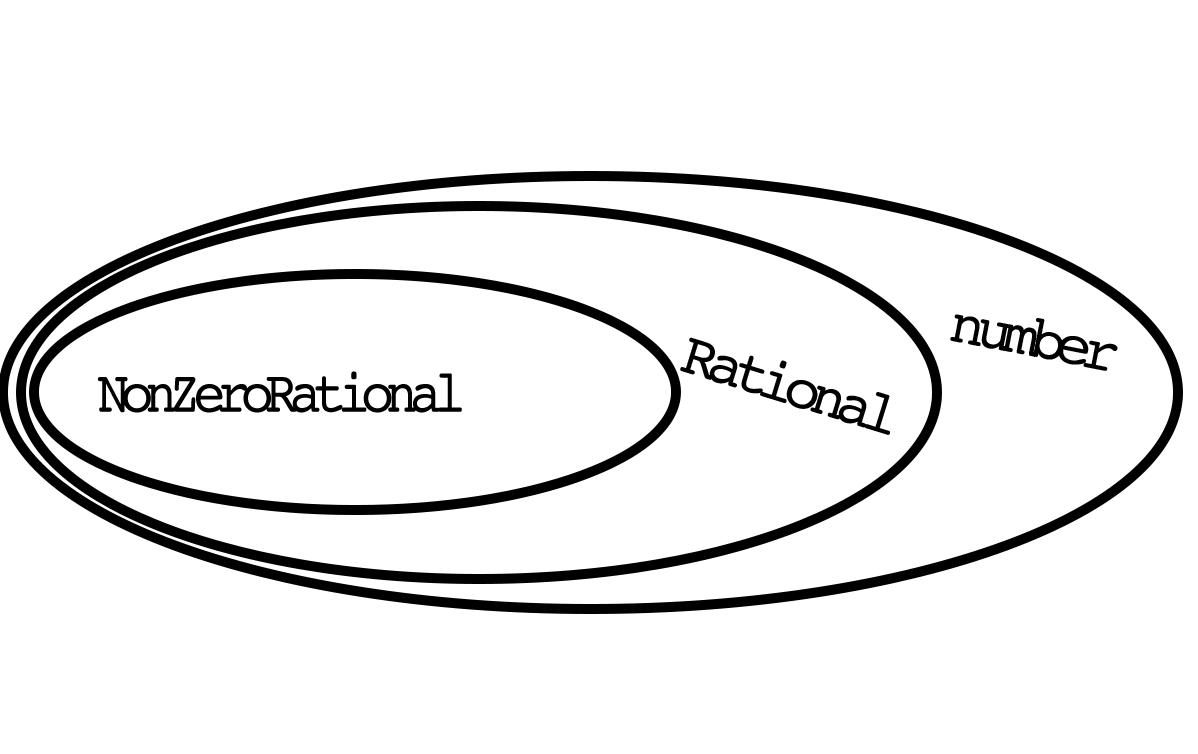
\includegraphics[width=7.1cm]{set_esimerkki}}
    \caption{Joukko NonZeroNumber on joukon number aito osajoukko}
    \label{fig:set-esimerkki}
\end{figure}

Joukkojen käyttöä voi pakottaa staattisella tyypityksellä. Ilman tyypityksen staattisuutta ohjelmoija ei helposti pysy määrätyissä raameissa \cite[44]{cantarella_fp_haitat}. Tyypit ohjaavat koodia ja estävät vääriä tiloja ohjemakoodin kääntämisvaiheessa.

Jos jakamisesimerkkiin saa määritettyä joukot funktion oikeiksi rajoiksi, on funktion väärinkäyttö mahdotonta. Avuksi tarvitsee tuoda \gls{ts}, \glsdisp{js}{JavaScriptin} päälle rakennettu ohjelmointikieli joka on tyypitetty \cite{typsecript_website}.

\begin{code}
    \begin{minted}{typescript}
type NonZeroNumber = number & {__brand: "nonzero"}
const isNonZeroNumber = (x:number): x is NonZeroNumber => x !== 0
\end{minted}
    \label{code:ts_set_theory_5}
    \caption{Joukon NonZeroNumber määrittäminen ja alkion sisältymisen tarkistaminen TypeScriptissä}
\end{code}

Tyyppi NonZeroNumber edustaa kaikkien ei-nolla-numeroiden joukkoa. Jos tyypin sijoittaa alkuperäiseen divide funktioon, on funktion väärinkäyttö mahdotonta. Kääntäjä pitää siitä huolen.


\begin{code}
    \begin{minted}{typescript}
const divide = (x:number) => (y:NonZeroNumber): number => x / y
\end{minted}
    \caption{Korrekti versio}
    \label{code:ts_set_theory_6}
\end{code}

Joukko-opin yhdistäminen ohjelmointiin ei ole ajattelutapa, joka rinnastetaan suoraan funktionaaliseen ohjelmointiin. Puhtaat funktiot ovat kuitenkin fundamentaalisesti aina siirtymisiä joukoista joukkoihin, on joukko-opin ajattelu vähintäänkin tervetullutta.



\subsection{Kategoriateoria}


Joukko-oppi ei ole ainoa ohjelmointiin sovellettava matemaattinen osa-alue. Funktionaaliselle ohjelmoinnille oleellisin osa-alue on \gls{category_theory} \cite{bartosz_category_for_progamers,promises-spec-94}.

Kategoriateoria tutkii matemaattisia rakenteita ja niiden välisiä suhteita erittäin abstraktilla tasolla. Se keskittyy objektien (kuten joukkojen tai tyyppien) ja niiden välillä olevien morfismien (funktioiden tai muunnosten) tutkimiseen. Kategoriateorian avulla voidaan ymmärtää ja formalisoida monimutkaisia matemaattisia ja ohjelmallisia rakenteita. \citep{bartosz_category_for_progamers,promises-spec-94,category_theory}

Kategoriateoria näkyy osittain myös JavaScriptissä, jossa Promise-luokka toimii lähes kuin \gls{monad}. Promise-luokka mahdollistaa asynkronisten operaatioiden ketjuttamisen ja virheiden käsittelyn tavalla, joka on verrattavissa kategoriateorian monadien tarjoamaan rakenteeseen. \citep{promises-spec-94}


% \begin{figure}[htbp]
% 	\centering
% 	\begin{tikzpicture}
% 		% Ellipses for sets A, B, and C with background colors
% 		\draw[thick, ellipse, fill=green!20] (0,0.5) ellipse (0.8cm and 2cm);  % Set A with light blue background
% 		\draw[thick, ellipse, fill=blue!20] (3,0.5) ellipse (0.8cm and 2cm); % Set B with light green background
% 		\draw[thick, ellipse, fill=red!20] (6,0.5) ellipse (0.8cm and 2cm);   % Set C with light red background

% 		% Nodes for set A (without borders)
% 		\node[draw=none] (A1) at (0,2) {1};
% 		\node[draw=none] (A2) at (0,1) {2};
% 		\node[draw=none] (A3) at (0,0) {3};
% 		\node[draw=none] (A4) at (0,-1) {4};

% 		% Nodes for set B (without borders)
% 		\node[draw=none] (B1) at (3,2) {1};
% 		\node[draw=none] (B2) at (3,1) {2};
% 		\node[draw=none] (B3) at (3,0) {3};
% 		\node[draw=none] (B4) at (3,-1) {4};

% 		% Nodes for set C (without borders)
% 		\node[draw=none] (C1) at (6,2) {1};
% 		\node[draw=none] (C2) at (6,1) {2};
% 		\node[draw=none] (C3) at (6,0) {3};
% 		\node[draw=none] (C4) at (6,-1) {4};

% 		% Arrows from A to B
% 		\draw[->] (A1) -- (B1);
% 		\draw[->] (A2) -- (B3);
% 		\draw[->] (A3) -- (B2);
% 		\draw[->] (A4) -- (B4);

% 		% Arrows from B to C
% 		\draw[->] (B1) -- (C2);
% 		\draw[->] (B2) -- (C1);
% 		\draw[->] (B3) -- (C3);
% 		\draw[->] (B4) -- (C4);

% 		% Labels for sets
% 		\node[draw=none, text=green!50!black] at (0,3) {$A = \{1,2,3,4\}$};
% 		\node[draw=none, text=blue] at (3,3) {$B = \{1,2,3,4\}$};
% 		\node[draw=none, text=red] at (6,3) {$C = \{1,2,3,4\}$};

% 		% Arrow to new diagram
% 		\draw[->, line width=1.5mm, black] (3,-1.75) -- (3,-2.75) node[midway, right] {};

% 		% New diagram with direct A to C composition
% 		% Ellipses for sets A and C below the original picture
% 		\draw[thick, ellipse, fill=green!20] (0,-4.5) ellipse (0.8cm and 2cm);  % Set A with light blue background
% 		\draw[thick, ellipse, fill=red!20] (6,-4.5) ellipse (0.8cm and 2cm);   % Set C with light red background

% 		% Nodes for set A (without borders) - Lower position
% 		\node[draw=none] (A1b) at (0,-3) {1};
% 		\node[draw=none] (A2b) at (0,-4) {2};
% 		\node[draw=none] (A3b) at (0,-5) {3};
% 		\node[draw=none] (A4b) at (0,-6) {4};

% 		% Nodes for set C (without borders) - Lower position
% 		\node[draw=none] (C1b) at (6,-3) {1};
% 		\node[draw=none] (C2b) at (6,-4) {2};
% 		\node[draw=none] (C3b) at (6,-5) {3};
% 		\node[draw=none] (C4b) at (6,-6) {4};

% 		% Direct arrows from A to C (composition)
% 		\draw[->] (A1b) -- (C2b);
% 		\draw[->] (A2b) -- (C3b);
% 		\draw[->] (A3b) -- (C1b);
% 		\draw[->] (A4b) -- (C4b);

% 	\end{tikzpicture}
% 	\caption{Funktioiden yhdistäminen joukko-opin näkökulmasta. Funktiot f : A$\,\to\,$B ja g : B$\,\to\,$C yhdistämällä saadaan g : A$\,\to\,$C.}
% \end{figure}

Lähestytään maailmaa, missä abstraktin taso nousee hyvin korkealle, jossa syvälliseen ymmärtämiseen vaaditaan korkeamman asteen matematiikan opintoja.

Luettaessa kategoriateoriaan liittyvää materiaalia, tai katsottaessa monia tunteja kategoriateoriaan liittyviä videoita, alkaa saamaan käsityksen siitä mitä kategoriateoria todellisuudessa on. Sen konkreettisesta käyttämisestä voi olla kuitenkin silti vaikea löytää sopivia tilanteita.

Ohjelmoinnin teoreettinen puoli on hyvä pitää mielessä, eikä sen opiskelusta missään nimessä ole haittaa. Kategoriateoria lienee mennä abstraktin tasollaan pidemmälle, kuin mitä JavaScript-kehittäjän tarvitsee tietää tavallisia ongelmia ratkaistaessa.

Jos ongelmat kuitenkin pystyy yleistämään oikealle tasolle, saa hyvässä tapauksessa monta voittoa, niin tehokkuuden kuin uudelleenkäytettävyyden piireissä \cite{clojure_compiler,bartosz_category_for_progamers}.


% \section{Tyypitys - todnäk rajaan ulos}

% TODO

% Tyypitys on todella tärkeää. Tyypit ohjaavat koodia ja estävät vääriä tiloja ohjemakoodin kääntämisvaiheessa. Tyypeillä pidetään ohjelmoija niissä raameissa, mitä funktionaalinen ohjelmointi usein vaatii \cite[44]{cantarella_fp_haitat}.

% JavaScriptissä tyypit eivät näy ohjelmoijalle muuten kuin sillon, kun ohjelma räjähtää ajon aikana. TypeScriptissä tyypit tulevat tielle. Haskelissa (ja PHP:ssa)

% TODO Mites \gls{js} :D

% \subsection{Staattinen ja dynaaminen tyypitys - todnäk rajaan ulos}

% TODO

% \subsection{Nimellinen ja rakenteellinen tyypitys - todnäk rajaan ulos}


% \subsection{Parametrinen polymorfismi - todnäk rajaan ulos}

% TODO

% Haskelille ominaista, fp ominaista.


% \subsection{Hindley-Milner tyyppijärjestelmä - todnäk rajaan ulos}

% TODO

% Feldmanin mukaan, mahdottomat tilat ovat testausta parempaa \cite{impossiblebetter}.

% Myös Dijkstran idis abstraktiosta sopii kauniisti tähän, ja esimerkki siitä et mitä fp on parhaimmillaan.

% Parametrinen polymorfismi näkyy täs myös.


\section{Pragmaattisuus}

Funktionaalisen ohjelmoinnin tärkein teoria alkaa olla käytynä. On aika tarkastella teoreettisella tasolla sitä, miten funktionaalinen ohjelmoinnin voi tuoda \gls{js} (ja \gls{ts}) arsenaaliin.

Kun funktionaalisen ohjelmoinnin kauneus on matemaattisissa kulmakivissä, joilla ei ole tapaa taipua, miten sen voi yhdistää säännöttömään JavaScriptiin tai muuhun vastaavanlaiseen kieleen?

Mikä on se lähestymistapa, jota tarvitaan käytännönläheiseen, pragmaattiseen, funktionaaliseen ohjelmointiin?

\subsection{Monadi on monoidi endofunktorien kategoriassa}

Monadi on monoidi endofunktorien kategoriassa on fraasi, jota käytetään humoristisesti yhteyksissä, missä pyritään selittämään funktionaalisen ohjelmoinnin matemaattisen osa-alueen kategoriateorian \gls{monad}-rakennetta \cite{bartosz_category_for_progamers_10}. Fraasi on surullisenkuuluisa, ja lienee yksi syy sille, miksei funktionaalinen ohjelmointi ole suositumpaa. Jos funktionaalisen ohjelmoinnin käsitteiden ymmärtämiseen tarvitsee useiden yliopistotasoisien kurssien taustatiedot, ei sopeutuminen ole helppoa.

Myöskin ohjelmoijat, jotka ovat tehneet kauan olio-ohjelmointia tai proseduraalista ohjelmointia, tahtovat toimia niillä tavoilla, mitä ovat oppineet. Esimerkiksi perustellaan niin, että JavaScript ei ole funktionaalinen ohjelmointikieli, vaikka siinä periaatteessa funktionaalista ohjelmointia voi kirjoittaakin. Tällaiset ongelmat tietysti ulottuvat pidemmälle kuin vain ohjelmointityyleihin. \citep{is_reduce_bad}

On harmillista perustella asioita pelkästään historiallisista syistä. Silloin ohjelmointikielet jäävät paikalleen \cite{promises-spec-94}.

\subsection{Funktionaalisen ohjelmoinnin ripottelu}

Kokemusten perusteella työpaikalla on havaittu funktionaalisen ohjelmoinnin paikallisuuden toimivan kohtuullisen hyvin muuten proseduraalisen ohjelmakoodin ympäristössä.

Robert C. Martinin mukaan pragmaattinen funktionaalinen ohjelmointi on sitä, että käytetään esimerkiksi \glsdisp{immutable_data}{muuttumattomuutta} ja puhtaita funktioita silloin, kun ne parantavat ohjelman luettavuutta, ylläpidettävyyttä ja suorituskykyä, ja kuitenkin niin, ettei vaadita täydellistä sitoutumista funktionaalisen ohjelmoinnin paradigmaan. \citep{martin2017pragmaticfp}

Myös Cantarella mainitsee opinnäytetyönsä loppupuolella ajatuksen, että mitä enemmän paradigmoihin liittyviin artikkeleihin perehtyy, sitä myötämielisemmäksi tulee ajatukselle, että paradigmoja tulisi yhdistellä vapaammin. \citep[45]{cantarella_fp_haitat}

Pragmaattista funktionaalista ohjelmointia vaikuttaa siis olevan se, että otetaan vain mitä tarvitaan. Toisaalta se, mitä tarvitaan ei ole välittömästi selvää.

\section{Funktionaalinen ohjelmointi \& Typescript}

TODO


% \begin{code}
% 	\begin{minted}{javascript}
% function rnd(min, max) { 
% 	return Math.floor(Math.random() * max) + min;
% }
% const rnd2 = (min, max) => Math.floor(Math.random() * max) + min;
% const rnd3 = min => max => Math.floor(Math.random() * max) + min;



% \end{minted}
% 	\caption{Kolme eri tapaa kirjoittaa funktio JavaScriptissä \cite{okhravi-g-discussion}. Funktiomäärittely, funktioilmaus ja osittain sovellettava funktioilmaus}
% 	\label{code:javascript_function_types}
% \end{code}

\subsection{Tyypitys \& joukko-oppi}

TODO

% Typescriptiä tullaan käyttämään insinöörityön koodiesimerkeissä, niin on aiheellista näyttää miten Typescriptissä fp näkyy.

% TODO TypeScript tyypit HYVÄ! Rich Hickey tykkää myös, voi tehä "product type" tms

% Toisaalta TS -> overhead, välillä joutuu kikkailemaan

% On huomattu, että JavaScript koodia kirjoittaessa voi olla vaikeaa pysytellä puhtaan funktionaalisen ohjelmoinnin raameissa, ja että usein olisi mielletysti helpompaa toteuttaa imperatiivisia ratkaisuja \cite[44]{cantarella_fp_haitat}.  LOLOL :D tää on just miks fp good

\subsection{Promise-tietorakenne ja osittaismonadisuus}

TODO

% Promise ei ole monadi :( \cite{read-it-later-11481,promises-spec-94}

% Se ei ole monadi, koska \gls{js} spesifikaatiota määriteltäessä ei päästy yhteisymmärrykseen siitä, että Promise-tietorakenteen tulisi olla monadi. Syy on moniuloitteinen, mutta pääasiallisesti sivuaa sitä, että funktionaalinen ohjelmointi ja sen käsitteet ovat vaikeita selittää kohtuullisella tarkkuudella. \citep{promises-spec-94}

% Tämä kirjoitushetkellä jo yli kymmenen vuotta sitten tehty päätös heikensi merkittävästi \gls{js}:n mahdollisuuksia viedä funktionaalista ohjelmointia eteenpäin. \Gls{js} kielenä on laajuudeltaan ongelmallinen. Uusia ominaisuuksia ei voi lisätä, jos vastaavanlaisia ominaisuuksia on aiemmin ollut osana suosittuja \gls{js}-kirjastoja \cite{proposal-joint-iteration,prototype_library_trends}.

% TODO lisää siitä että ei tulla ikinä saamaan "builtin" monadeja
% TODO myös että no mitä se tarkoittaa, onko juuri promisen kannalta mitään merkitystä

\subsection{Ramda.js}

% Koska funktionaalisen ohjelmakoodin tuottaminen \gls{js} tai \gls{ts} ympäristössä enemmän tai vähemmän vaatii jotain kirjastoa, joko itse ohjelmoitua tai ulkoista, niin tähän insinöörityöhön on kirjastoksi valittu Ramda.js.

% Ramda.js, ja kirjaston taustalla oleelinen Fantasy Land -algebrallinen spesifikaatio, ovat kirjastoja jotka pyrkivät johdonmukaiseen funktionaaliseen ohjelmointiin JavaScriptissä. Näiden kirjastojen kehittäjistöstä löytyy samoja henkilöitä jotka aikoinaan pyrkivät saamaan Promise-tietorakenteen virallisesti monadiseksi \cite{ramda:contributors,fantasy-land:contributors,promises-spec-94}. Näyttää siltä, että kun tähän tavoitteeseen ei päästy, päättivät kehittäjät tuoda funktionaalisen ohjelmoinnin JavaScriptiin omin keinoin.

% TODO miten ramda toimii

% TODO miten ramda sopii omien funktioiden kanssa

% TODO miten typescript? ei hyvä, tyypit ovat mitä sattuu (kokemuspohjaisesti)

\subsection{Rajoitteet}

TODO

% Mitkä asiat eivät ole mahdollisia, tai mitkä ovat erittäin hankalia / järjettömiä kun ohjelmoidaan fp koodia \gls{ts}-maailmassa.


\section{Vertailu yhteenvetona}

TODO

% Ehkä nopea yhteenveto että mikä on täysin fp ominaista ja mikä ei. Mahdollisesti jokin kiva taulukko.